\documentclass[]{article}
\usepackage{amsmath}
\usepackage{amsfonts} 
\usepackage[english]{babel}
\usepackage{amsthm}
\usepackage{mathtools}
\usepackage{hyperref}
\usepackage{bbm}  % for indicator functions and stuff. 
\usepackage{amssymb}
% \usepackage{minted}
% Basic Type Settings ----------------------------------------------------------
\usepackage[margin=1in,footskip=0.25in]{geometry}
\linespread{1}  % double spaced or single spaced
\usepackage[fontsize=12pt]{fontsize}

\theoremstyle{definition}
\newtheorem{theorem}{Theorem}       % Theorem counter global 
\newtheorem{prop}{Proposition}[section]  % proposition counter is section
\newtheorem{lemma}{Lemma}[subsection]  % lemma counter is subsection
\newtheorem{definition}{Definition}
\newtheorem{remark}{Remark}[subsection]


\hypersetup{
    colorlinks=true,
    linkcolor=blue,
    filecolor=magenta,
    urlcolor=cyan,
}
\usepackage[final]{graphicx}
\usepackage{listings}
\usepackage{courier}
\lstset{basicstyle=\footnotesize\ttfamily,breaklines=true}
\newcommand{\indep}{\perp \!\!\! \perp}
\usepackage{wrapfig}
\graphicspath{{.}}
\usepackage{fancyvrb}

%%
%% Julia definition (c) 2014 Jubobs
%%
\usepackage[T1]{fontenc}
\usepackage{beramono}
\usepackage[usenames,dvipsnames]{xcolor}
\lstdefinelanguage{Julia}%
  {morekeywords={abstract,break,case,catch,const,continue,do,else,elseif,%
      end,export,false,for,function,immutable,import,importall,if,in,%
      macro,module,otherwise,quote,return,switch,true,try,type,typealias,%
      using,while},%
   sensitive=true,%
   alsoother={$},%
   morecomment=[l]\#,%
   morecomment=[n]{\#=}{=\#},%
   morestring=[s]{"}{"},%
   morestring=[m]{'}{'},%
}[keywords,comments,strings]%
\lstset{%
    language         = Julia,
    basicstyle       = \ttfamily,
    keywordstyle     = \bfseries\color{blue},
    stringstyle      = \color{magenta},
    commentstyle     = \color{ForestGreen},
    showstringspaces = false,
}



\begin{document}
\section{Notations}
\begin{enumerate}
    \item [1.)] $\text{cvxh}$ denotes the convex hull of some sets in Euclidean space. 
    \item [2.)] $\mathbbm 1_M$ denotes that activation vector defined by the set $M$; $(\mathbbm 1_M)_e = 1 \iff e\in M$; else $(\mathbbm 1_M)_e = 0\iff e\not\in M$. 
    \item [3.)] Bold face $\mathbf 1, \mathbf 0$ denotes a vector full of ones and zeros, the size of them depends on the context, if ambiguity arised, a subscript will be there denoting the size. 
    \item [4.)] We define the set of edges pointing out of a vertex $v$ on a digraph to be $\delta^+(v)$, and the set of edges pointint into the vertex as $\delta^{-}(v)$. It's like flux, but on the vertex. 
\end{enumerate}
\numberwithin{equation}{subsection}
\section{Problem 8.12}
    \begin{prop}[Non Bipartite Matching]
        Let $G=(V, E)$ be a non-bipartite graph. Show that the inequalities (LP formulations of the matching problem) are not enough t define the matching polytope. Mathematically Speaking: 
        \begin{align}
            P:=\text{cvxh}\{\text{All Matching }\mathbbm 1_M \text{on G}\} \subsetneqq Q:=\{x\ge \mathbf 0 \;| Ax \le \mathbbm 1\}
        \end{align}
    \end{prop}
    \subsection{Proof Strategies}
        The inequality can be proved by choosing one element $x\in P$ such that it's not in $Q$. We make use of the fact that a graph is non-bipartite iff it has odd cycles in it. 
        \par
        Denote $C$ to be the set of edges that describes the odd cycle on $G$. 
    \subsection{The Proooooo0000oooooOWOOOf}
    \begin{proof}
        Choose an element $x\in P$ we have: 
        \begin{align}
            \mathcal M &:= \{\text{All Integral Matching on G}\}
            \\
            x &= \sum_{M\in \mathcal M}^{}
                \lambda_i\mathbbm 1_M;
                \quad 
                \langle \mathbbm 1, \vec{\lambda}\rangle = 1, \vec \lambda \ge \mathbf 0
            \\
            \forall e \in E: x_e &= \sum_{M\in \mathcal M}^{}\lambda_i (\mathbbm 1_M)_e
                \quad 
                \langle \mathbbm 1, \vec{\lambda}\rangle = 1, \vec \lambda \ge \mathbf 0
        \end{align}
        The first line decribes that the vector $x$ is a convex combinations of all indicator vectors of a matching on the graph. The next line highlights the fact that, for all edges $e$ on the cycle, it's still a convex combinations of the subset of elements in $\mathbbm 1_M$ selected by $M$. 
        \par
        Now I am going to choose another element $x^+\in P$ such that it's not in $Q$. define this element to be: 
        \begin{align}
            \forall e \in E:\; (x^+)_e := \begin{cases}
                \frac{1}{2} & e \in C
                \\
                0  & \text{else}
            \end{cases}
        \end{align}
        $x^+ \in Q$ because $\forall v\in V: \sum_{v\ni e}^{}x_e = 1 \le 1$, and $\forall v \in V\setminus C: \sum_{e \ni v}^{}x_e = 0\le 1$. Observe that if I sum up all $(x^+)_e$ for all $e\in C$, we have: 
        \begin{align}
            \sum_{e\in C}^{}(x^+)_e = \langle \mathbbm 1_C, x^+\rangle = \frac{(2n + 1)}{2} = n + \frac{1}{2}
        \end{align}
        Here, we assume that the odd cycle have length $2n + 1$. Now, for any element $x\in P$, we can sum up edges only on cycle $C$ too, obtaining: 
        \begin{align}
            \langle \mathbbm 1_C, x\rangle 
            &= 
            \left\langle 
                \mathbbm 1_C, 
                \sum_{\forall M}^{}\lambda_i \mathbbm 1_M
            \right\rangle
            \\
            &= \sum_{\forall M\in \mathcal M}^{}
                    \lambda_i \langle\mathbbm 1_M,\mathbbm 1_C\rangle = 
                \sum_{\forall M\in \mathcal M}^{}
                    \lambda_i \mathbbm 1_{M\cap C} \le n
        \end{align}
        The above expression denotes the fact that, if we zoom into the odd cycle and exam the matching on the odd cycle, then their convex combinations is going to be always less than $n$. This is true because $M$ on $C$ have a maximum assignment of $n$ edges, more than that it won't be a matching. The weighted sum of $\lambda_i$ preserves the bound (summation is a linear transform). Which is impossible to represent $x^+\in Q$ (it sums up to $n + 1/2$, which is more). Therefore, we have proven the fact that $P\subsetneqq Q$. 
    \end{proof}


\section{Problem 8.14}
    \begin{prop}
        The stable set polytope $P_{\text{stable}}$ of $G:= (V, E)$ is the convex hull of the incidence vectors of the stable set in $G$, give a description of the linear inequalities defining the stable set of the polytope of a bipartite graph $G$. 
    \end{prop}
    \subsection{Proof Strategies}
        The polytope would need the help of a incidence matrix $A$ for the graph $G$. The indicence matrix is a $|V|\times |E|$ defined as: 
        \begin{align}
            A_{v, e}:= \begin{cases}
                1 & v\in e
                \\
                0 & \text{else}
            \end{cases}
        \end{align}
        Then, for all independent sets on a graph, it will fall into the following linear program: 
        \begin{align}
            x&\in \mathbb R^{|V|}    
            \\
            A^Tx &\le \mathbf 1
        \end{align}
        Observe that for all $v$, $(A^Tx)_v = \sum_{v\ni e}^{}1$, which counts the total number of edges incident to the vertex $v$. All independent set $F$ has incidator $\mathbbm 1_F$ will satisfies this condition. 
    \subsection{The ProooOooOOooF}
    \begin{proof}
        Recall: Theorem 8.3 that the incidence matrix $A_G$ for a bipartite graph is total unimodular. Then $A^T$ is T.U as well therefore, the polytope $P:=\{x\ge \mathbf 0: A^Tx\le \mathbf 1\}$ is integral. All stable set vector $\mathbbm 1_F \in P$ and this is direct from its definition. Then any convex combinations of $\mathbbm 1_F$ will be $\in P$. Therefore $P_{\text{stable}}\subseteq P$ . 
        \par
        For all integral vectors inside $P$, it has to be $\mathbbm 1_F$ where $F$ is an independent set. A polytope is defined as the convex hull of all its vertices(In this case, $P$ has all integral vertices). Therefore all its vertices are describing an independet set as well, therefore $P = P_{\text{stable}}$. 
    \end{proof}

\section{Problem 4.5}
    \begin{prop}
        Let $D:(V, A)$ be a digraph, set $s, t\in V$ to be the source and sink for a networkflow, then define flow $f: A\mapsto \mathbb R_+$ as the $s-t$ flow of value $\beta$. How that $\exists f': A\mapsto \mathbb Z_+$ of value $\lceil \beta\rceil$ such that $\lfloor f(a)\rfloor \le f'(a) \le \lceil f(a)\rceil$. 
    \end{prop}
    \subsection{Proof Strategies}
        The problem can be viewed as looking for a flow that is $\lfloor f\rfloor\le x \le \lceil f\rceil$ ($f$ is the flow vector $f\in \mathbb R^{|A|}$, $f_a = f(a)$) such that it sends exactly a flow of $\lceil \beta \rceil$. This is always possible because rounding up $f$ to attain something $\ge \lceil f\rceil$. Therefore, we always have a solution for $x$, but the problem is, is it neccessarily integral? 
        \par
        To do that we make use of total unimodularity of matrices. Notation wise we use $\mathbf e_k$ to denote the standard basis vectors. 
    \subsection{The proof}
    \begin{proof}
        Define the flow digraph matrix $A$: 
        \begin{align}
            A = \begin{bmatrix}
                \mathbbm{1}_{\delta^+(s)} - \mathbbm{1}_{\delta^{-}{(s)}}
                \\
                \mathbbm{1}_{\delta^+(t)} - \mathbbm{1}_{\delta^{-}{(t)}}
                \\
                \mathbbm{1}_{\delta^+(v_1)} - \mathbbm{1}_{\delta^{-}(v_1)}
                \\
                \vdots
                \\
                \mathbbm{1}_{\delta^+(v_n)} - \mathbbm{1}_{\delta^{-}(v_n)}
            \end{bmatrix}
        \end{align}
        The first row and the second row are edges that are coming in and out of the source and the sink vertex. I want the flow coming in and out to be $\lceil \beta \rceil$, then we consider: 
        \begin{align}
            Ax = \lceil \beta\rceil(\mathbf e_1 -\mathbf e_2)
        \end{align} 
        To assert the conditions that $\lfloor f\rfloor\le x \le \lceil f\rceil$ we have: 
        \begin{align}
            & 0 \le x - \lfloor f \rfloor\le \lceil f\rceil
            \\
            & x - \lfloor f \rfloor + s = \lceil f \rceil \quad s \ge \mathbf 0, x\ge \mathbf 0
            \\
            & x + s = \lceil f \rceil - \lfloor f \rfloor \quad s, x\ge \mathbf 0
        \end{align}
        Then, we have the following polytope to deal with: 
        \begin{align}
            \underbrace{\begin{bmatrix}
                A & \mathbf 0
                \\
                I & I 
            \end{bmatrix}}_{=:B}\begin{bmatrix}
                x \\ s
            \end{bmatrix} = 
            \underbrace{\begin{bmatrix}
                \lceil \beta \rceil (\mathbf e_1 -\mathbf e_2)
                \\
                \lceil f \rceil - \lfloor f \rfloor
            \end{bmatrix}}_{=: b}
        \end{align}
        The claim is that, the 2 by 2 block matrix above is totally unimodular, and because its totally unimodular, it's unimodular, in additoin, $A$ the incidence matrix will be full rank when $G$ is connected(It will be, if not, we can remove all the edges that has $f=0$, then we are left with a graph connected by the defined real flow $f$). By theorem 8.2 we proved in class, we have the fact that the polytope $\{x\ge \mathbf 0| Bx = b\}$ is integral. We know it's definitely non-empty, therefore, an integral flow $x$ exists and it is in between $\lfloor f \rfloor, \lceil f\rceil$ for all the arcs in the graph. 
        \\
        The 2 by 2 is unimodular, we denote any submatrices using the $\tilde.$ decorator. Then any square sub matrix of $B$ can be written in the form of: 
        \begin{align}
            \text{det}\begin{bmatrix}
                \tilde{A} & \mathbf 0
                \\
                \tilde{I} & \tilde{I}
            \end{bmatrix}
            =
            \text{det}(\tilde{A})\text{det}(\tilde{I}) 
            \in \{\pm 1, 0\}
        \end{align}
        We use the theorem that, for any block diagonal matrix, its determiannt is the product of the determinant of all its block matrices on its diagonal (I learned this in a numerical linear algebra class); any submatrix of $I$ is going to be either $0$ or $1$, therefore, the product of this square sub matrix is still, $\pm 1, 0$. It's T.U. 
    \end{proof}
    
\section{Problem 4.7 (ii)}
    \begin{figure}
        \centering
        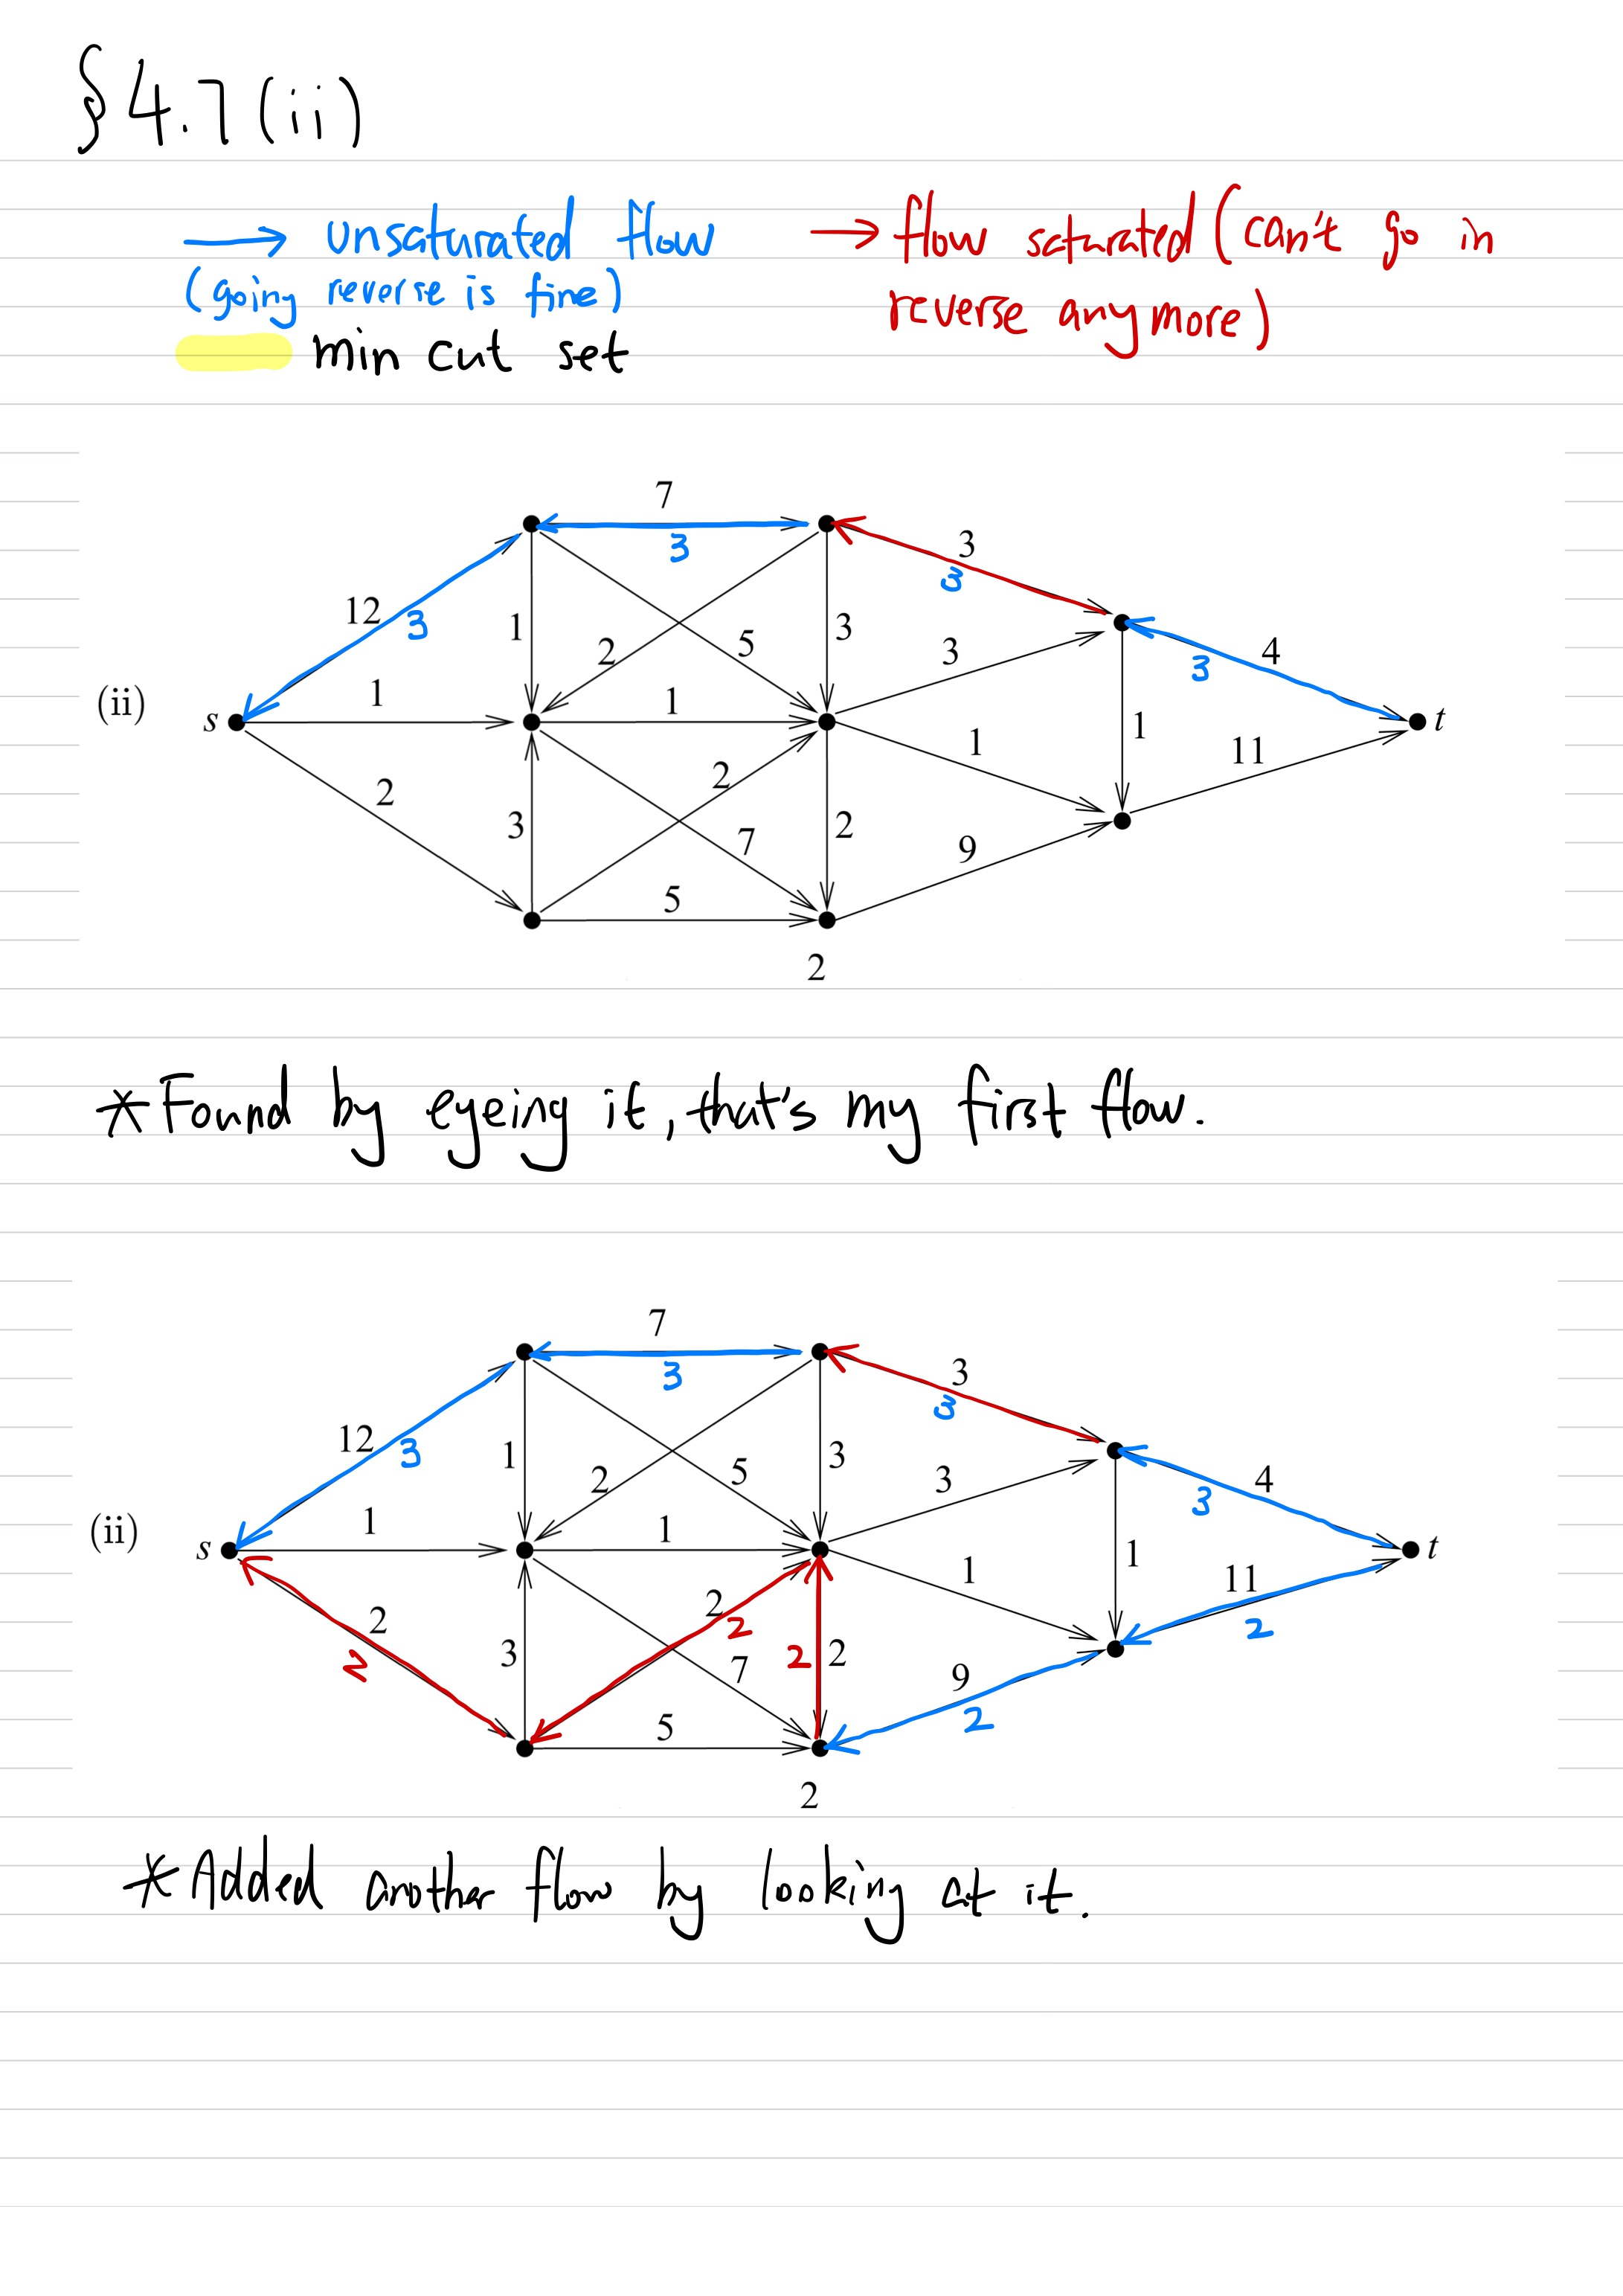
\includegraphics[width=16cm]{HW6-7.jpg}    
    \end{figure}

    \newpage
    \begin{figure}
        \centering
        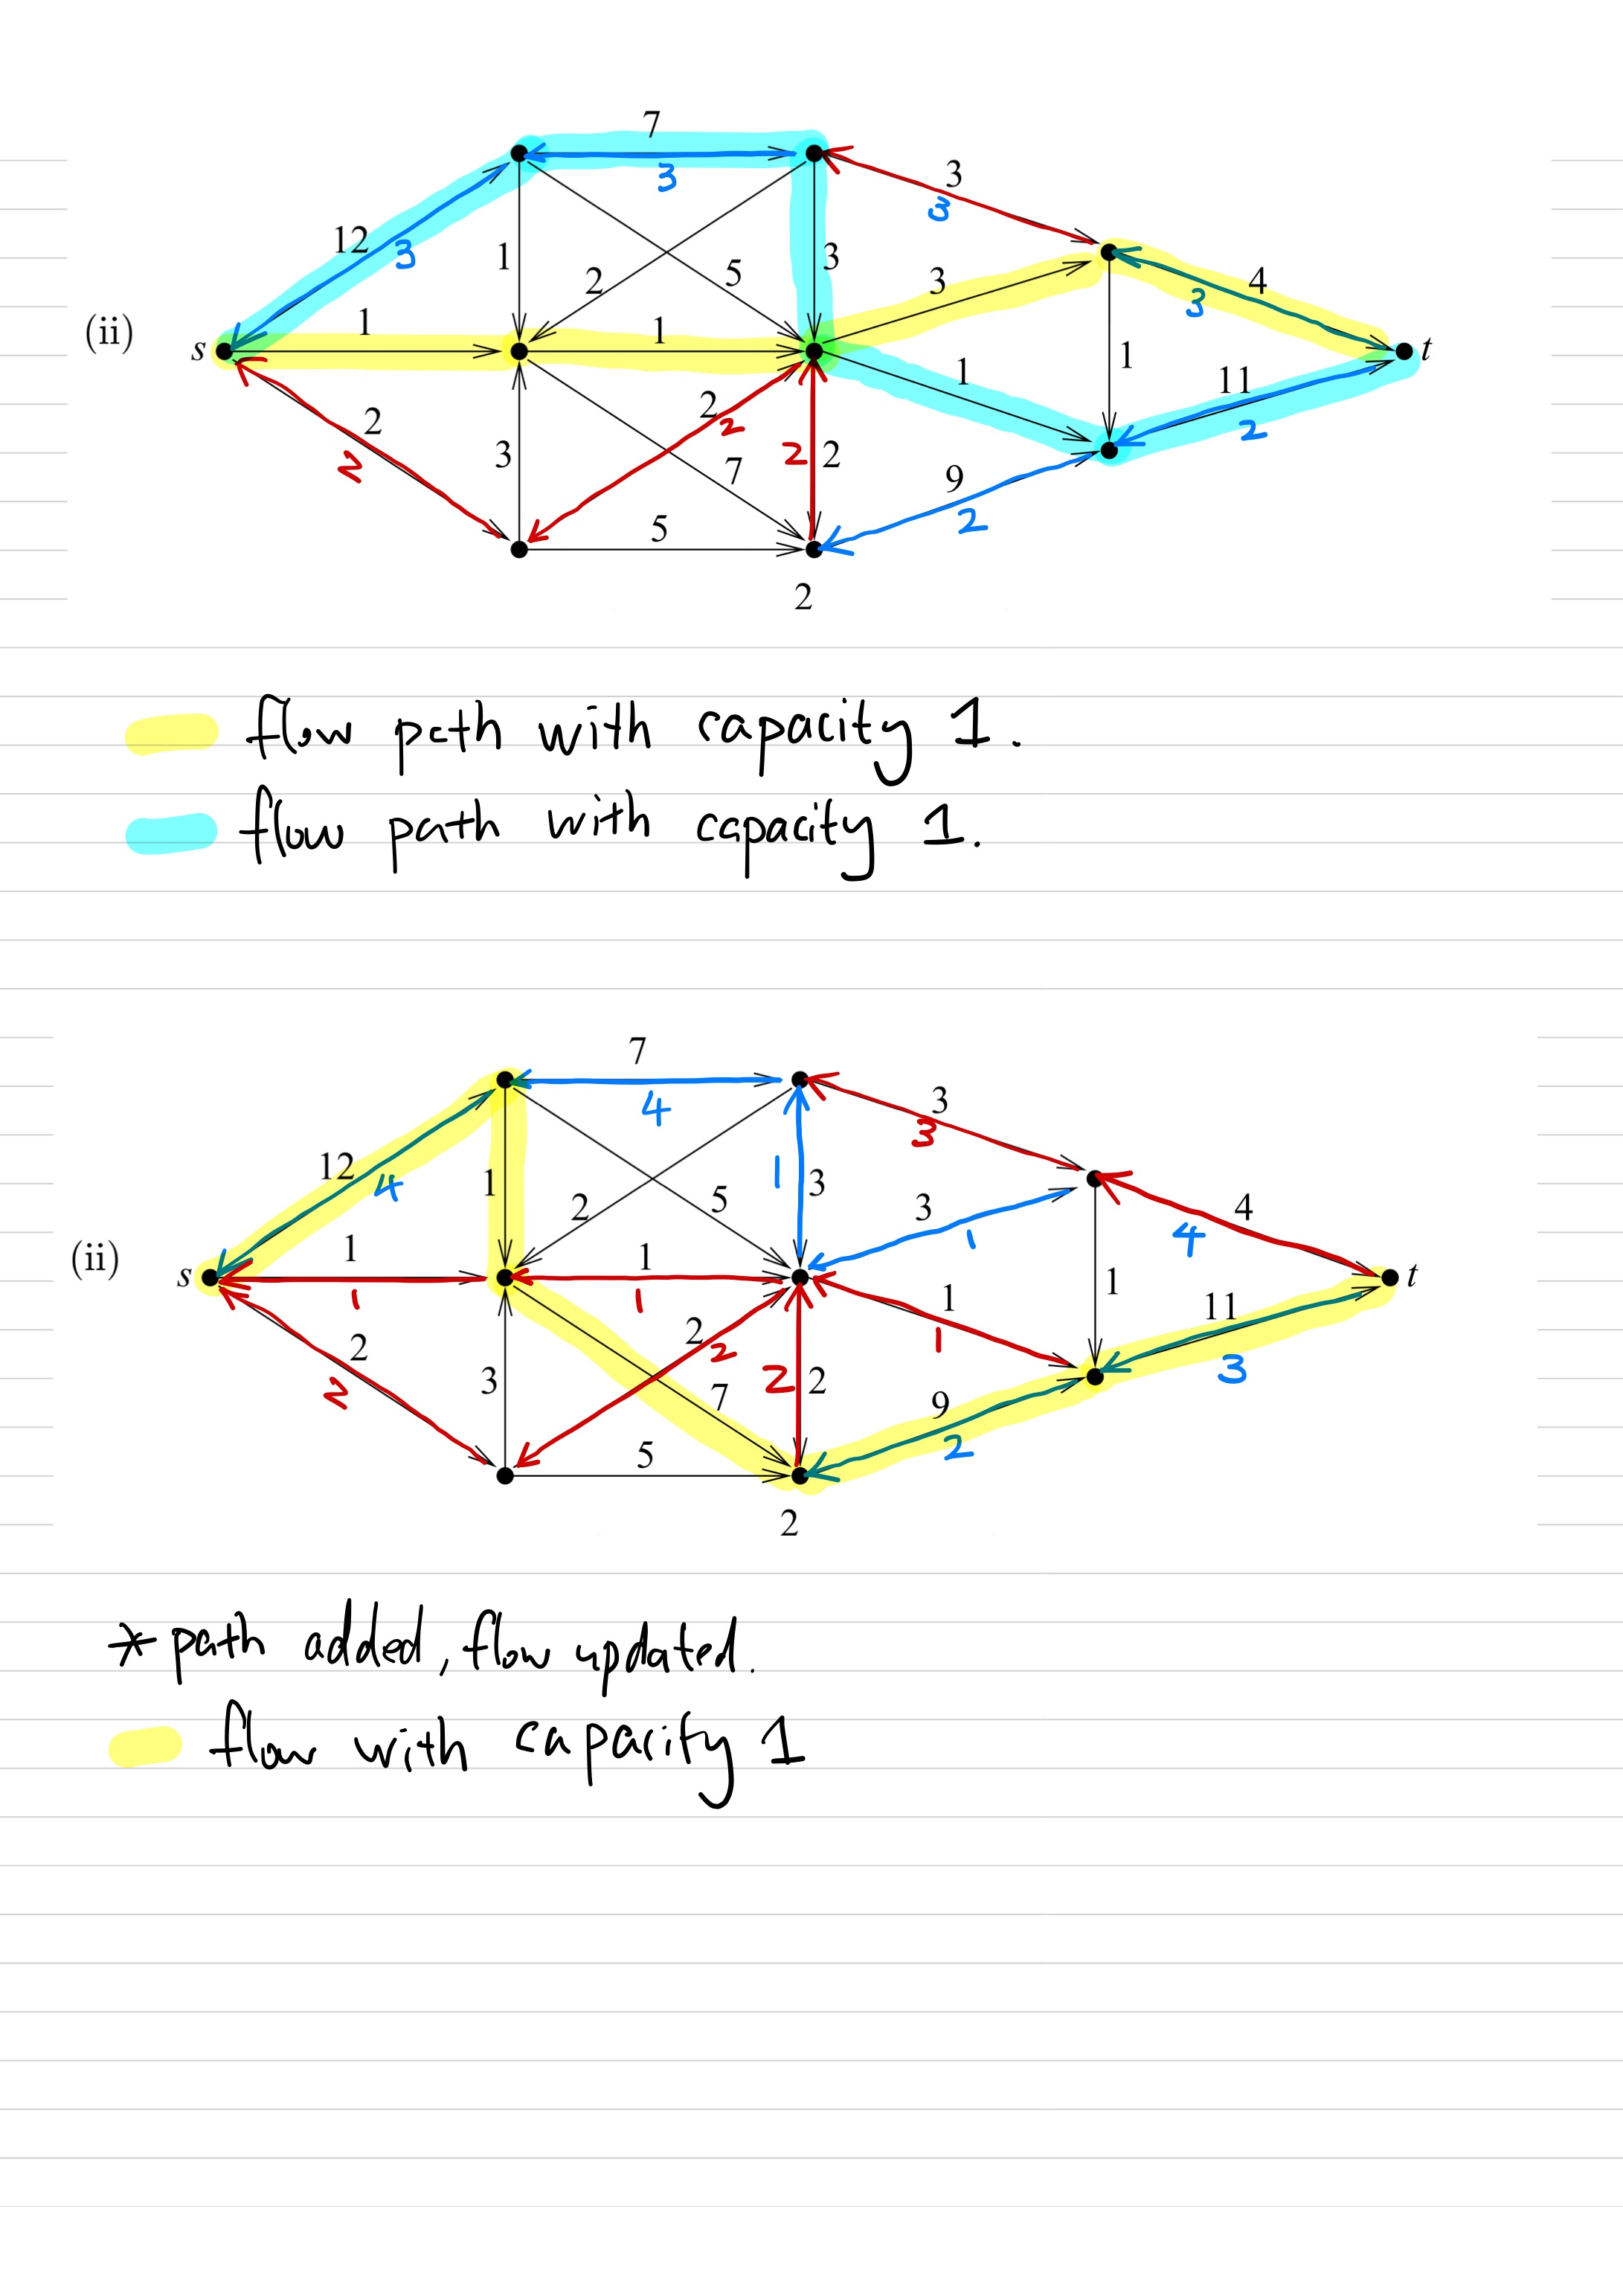
\includegraphics[width=16cm]{HW6-8.jpg}    
    \end{figure}
    
    \newpage
    \begin{figure}
        \centering
        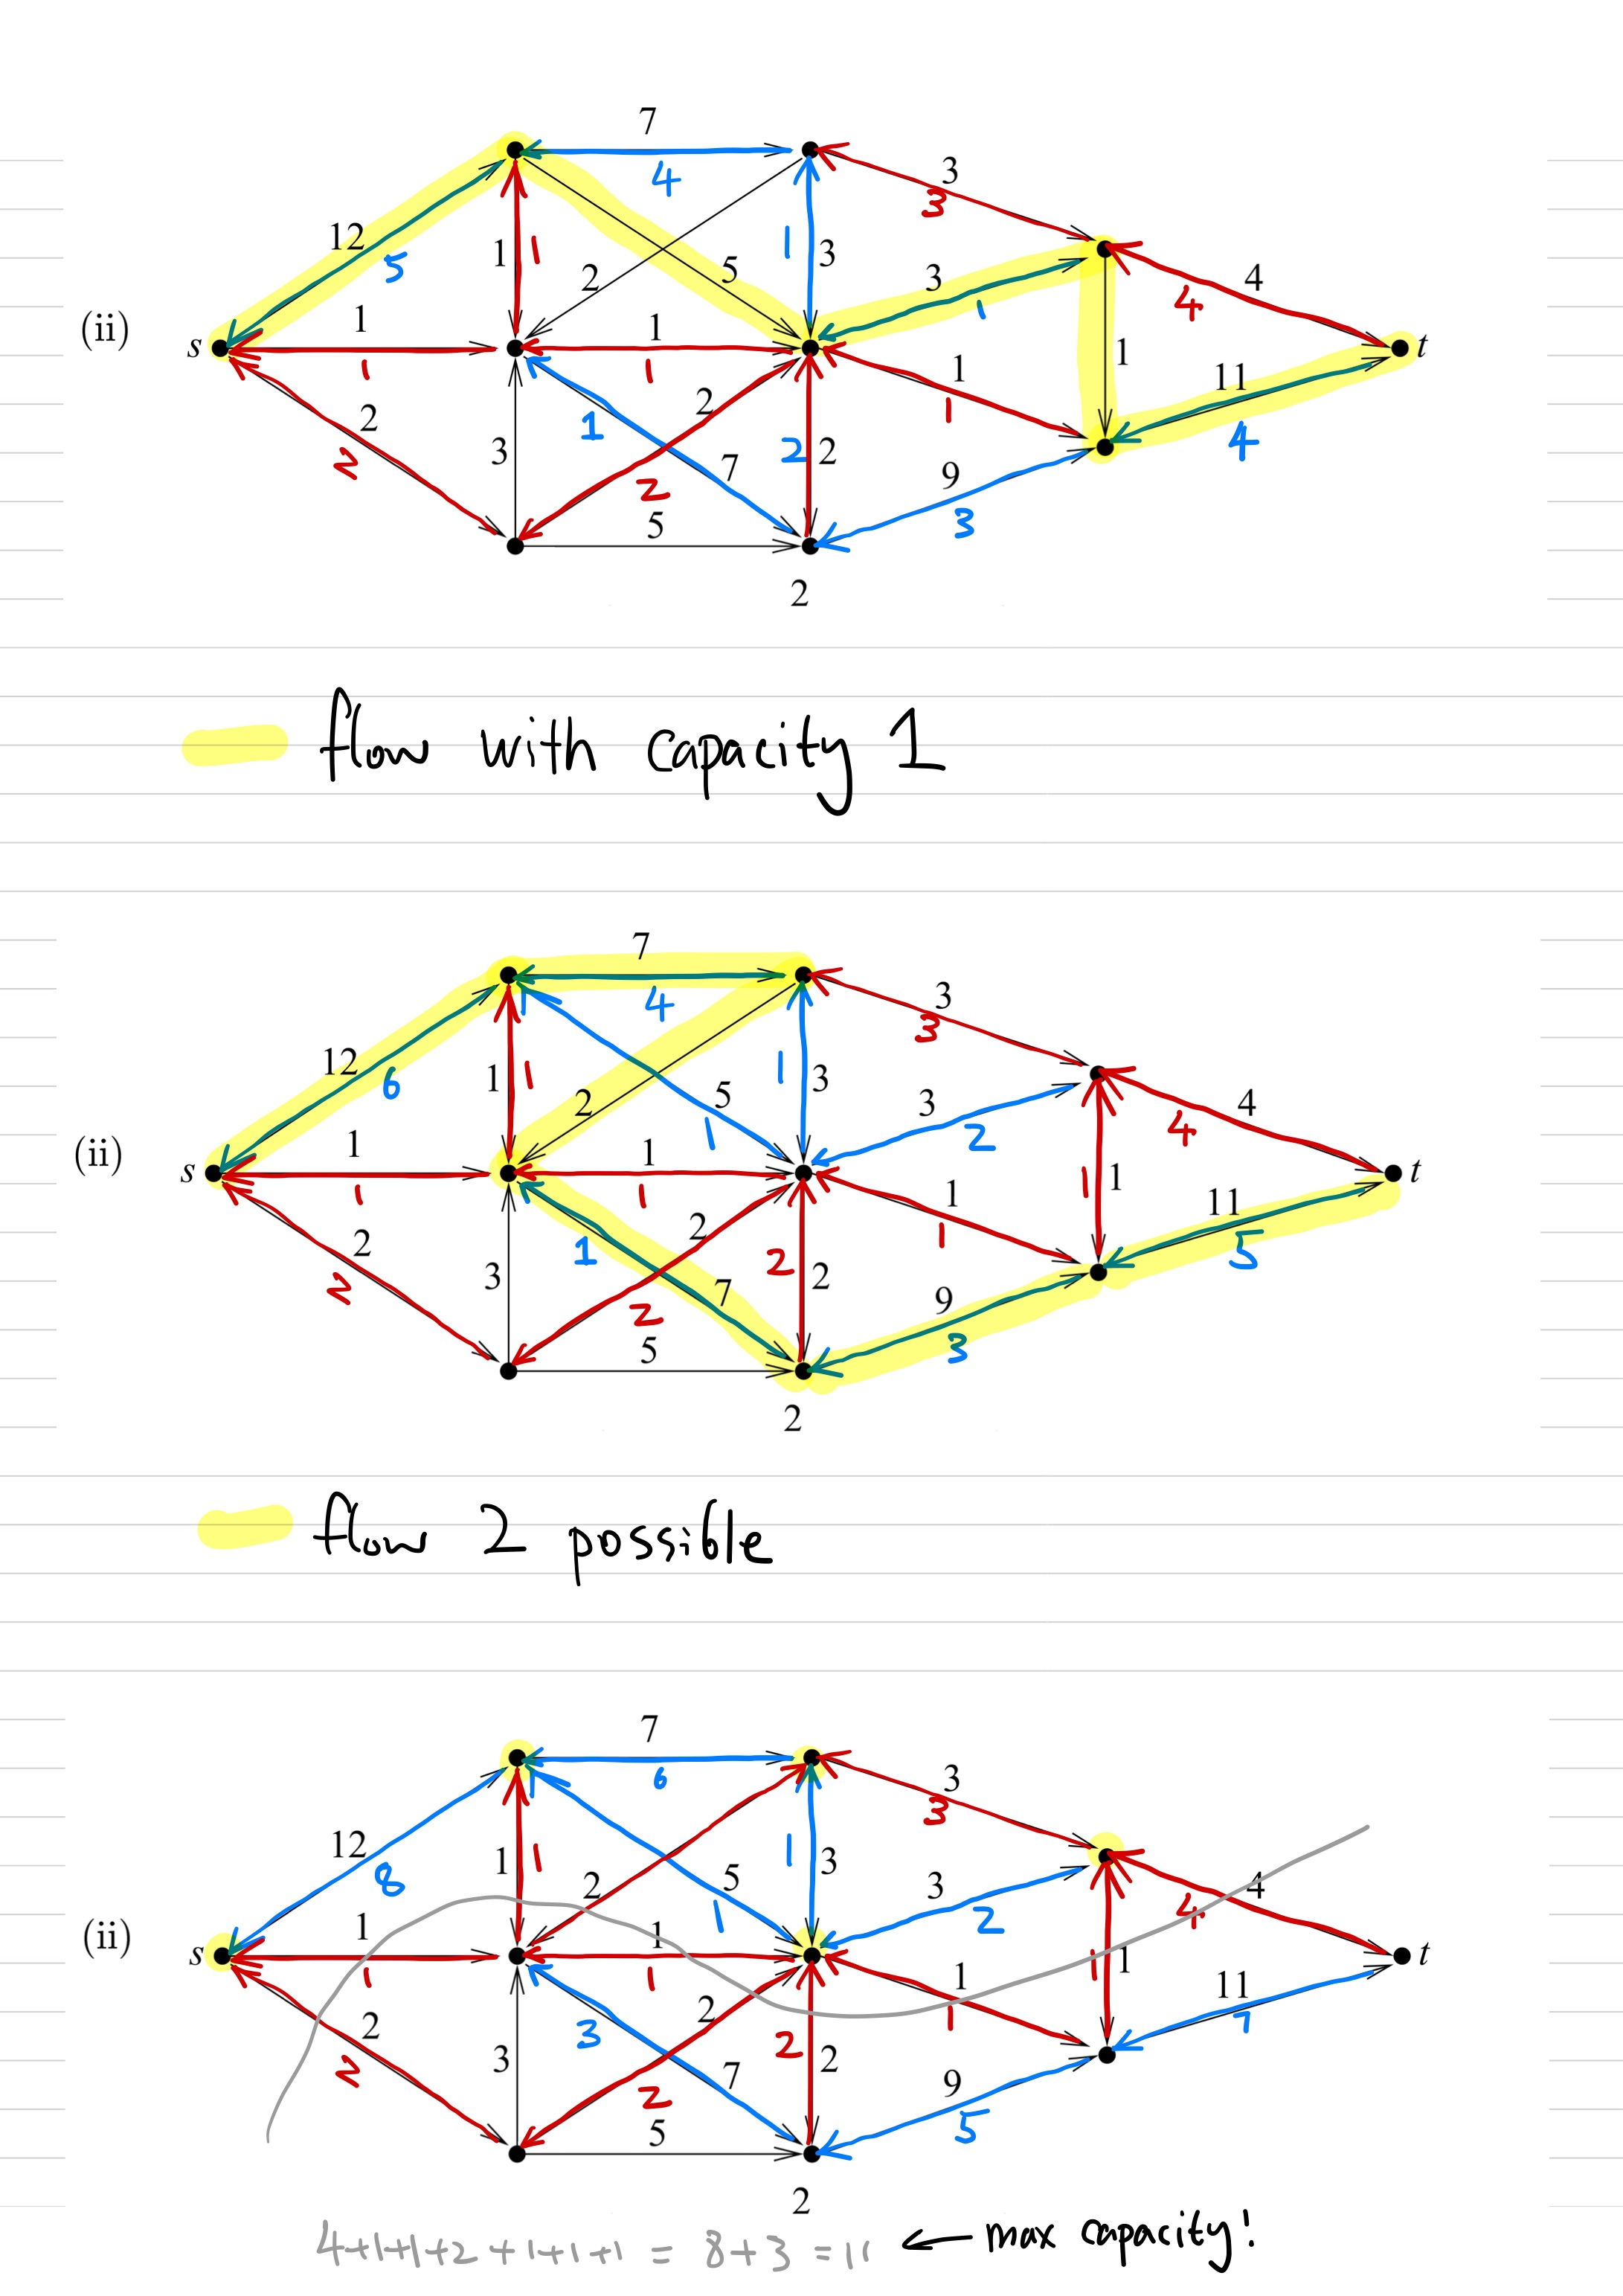
\includegraphics[width=16cm]{HW6-9.jpg}    
    \end{figure}
    

\end{document}